\paragraph{4. Do the lost relations result in New Observable Behaviors?}

        To answer this, we need to see whether the relations removed had an impact on possible $\stck{_{rf}}$ relations other than those with $e$. 
        We divide our argument into two parts, viz. the two types of relations removed:
        \begin{tasks}(2)
            \task $\reln{k}{hb}{R_{uo}}$. 
            \task $\reln{R_{uo}}{hb}{k}$.
        \end{tasks}

        Figure~\ref{elim_read:case1} shows a breakdown of sub-cases for case (a), varying based
        on the nature of event $k$.
        \begin{figure}[H]
            \centering
            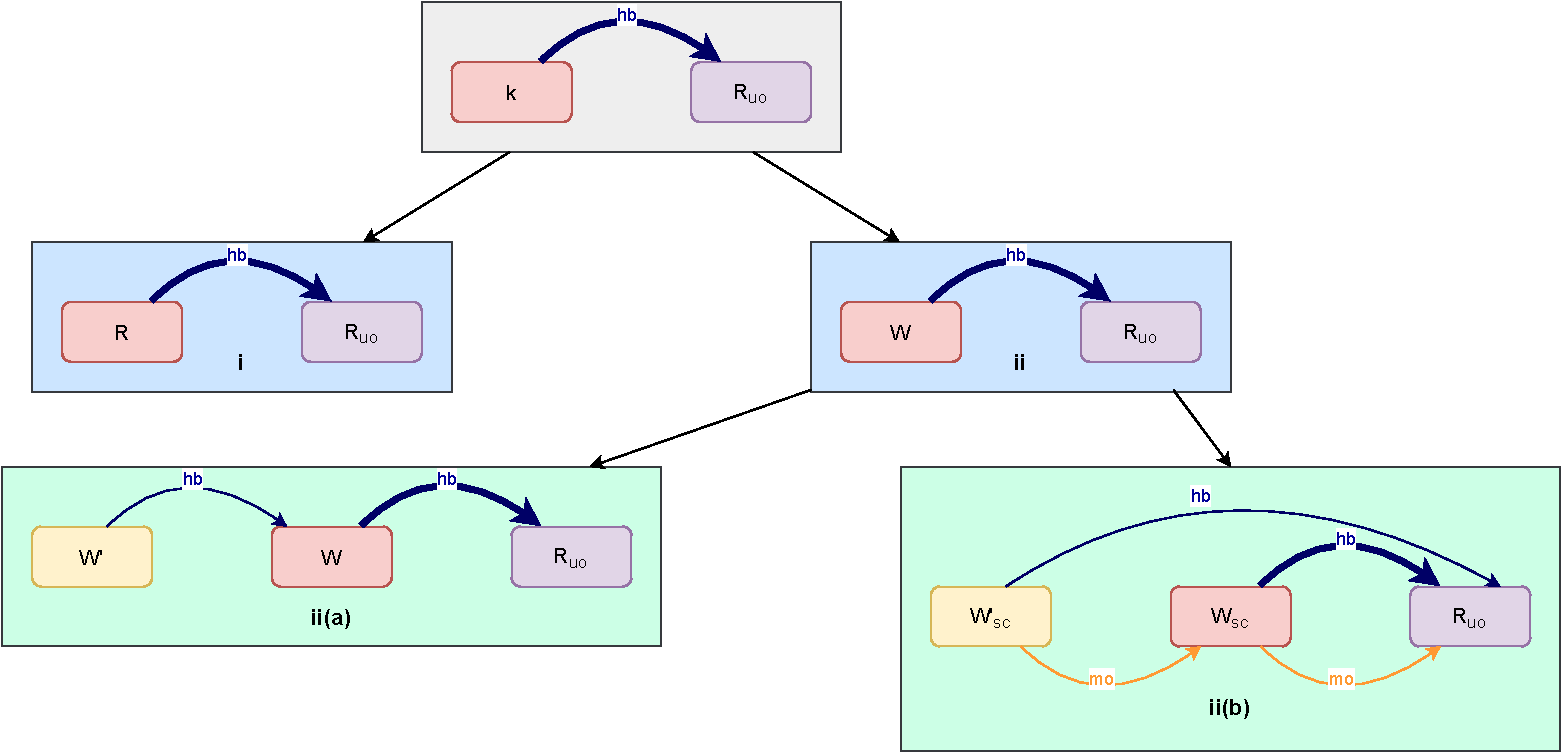
\includegraphics[scale=0.5]{5.Elimination/1.ValidEliminationCandidate/ReadElimProof/ProofParts/Part4_Case1.pdf}
            \caption{The impact of lost relation $\reln{k}{hb}{R_{uo}}$ on observable behaviors.}
            \label{elim_read:case1}
        \end{figure}

        Observations:
        \begin{itemize}
            \item (i) is not a pattern forbidden by the consistency rules.
            \item (ii)(a) is a pattern of Axiom \ref{CoRe}, however, only restricting $\stck{_{rf}}$ relation with $R$ and $W'$(which here is our Unordered Read)
            \item (ii)(b) is a pattern of Axiom \ref{SeqCsAt}, however, once again, only restricting $\stck{_{rf}}$ relation with $R$ and $W'$. 
        \end{itemize}

        Figure~\ref{elim_read:case2} shows a breakdown of sub-cases for case (b), varying based
        on the nature of event $k$.
        \begin{figure}[H]
            \centering
            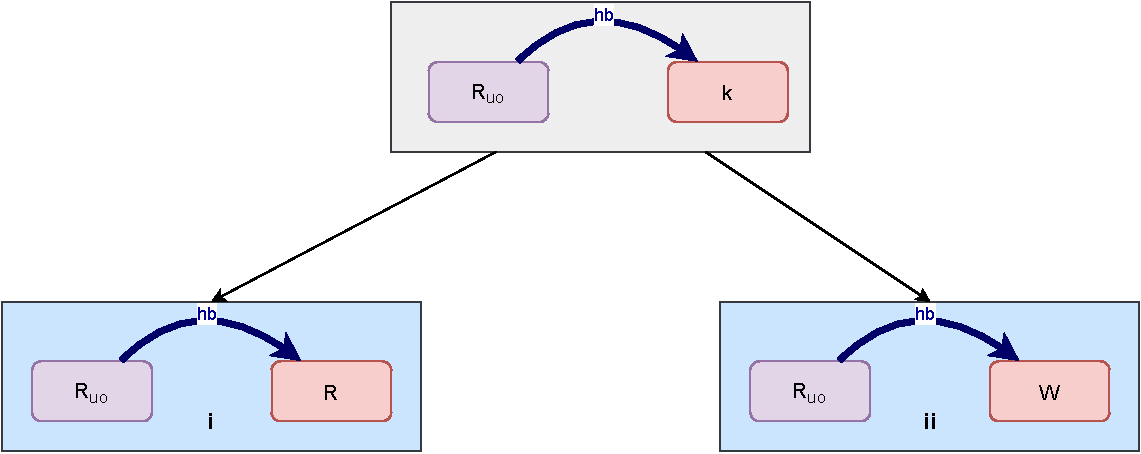
\includegraphics[scale=0.5]{5.Elimination/1.ValidEliminationCandidate/ReadElimProof/ProofParts/Part4_Case2.pdf}
            \caption{The impact of lost relation $\reln{R_{uo}}{hb}{k}$ on observable behaviors.}
            \label{elim_read:case2}
        \end{figure}

        Observations:
        \begin{itemize}
            \item (i) is not a pattern in any Consistency rules
            \item (ii) is a pattern of Axiom \ref{CoRe}, however, only restricting $\stck{_{rf}}$ relation with $R$ and $W$
        \end{itemize}

        From the above observations, we can infer that the relations removed only have restriction on reads-from relations on the event $e$ we eliminate. 
        Thus, we can conclude that no new observable behaviors are introduced due to the removed $\stck{_{hb}}$ relations. 